\documentclass[12pt]{beamer}
\newenvironment{ConCodigo}[1]
  {\begin{frame}[fragile,environment=ConCodigo]{#1}}
  {\end{frame}}
\graphicspath{{Imagenes/}{../Imagenes/}}
\usepackage[utf8]{inputenc}
\usepackage[spanish]{babel}
\usepackage{hyperref}
\usepackage{etex}
\reserveinserts{28}
\usepackage{amsmath}
\usepackage{amsthm}
\usepackage{mathtools}
\usepackage{multicol}
\usepackage{multirow}
\usepackage{tabulary}
%\usepackage{tabularx}
\usepackage{booktabs}
\usepackage{nccmath}
\usepackage{biblatex}
\usepackage{epstopdf}
\usepackage{graphicx}
\usepackage{siunitx}
\sisetup{scientific-notation=true}
%\usepackage{fontspec}
\usepackage{lmodern}
\usepackage{float}
\usepackage[format=hang, font=footnotesize, labelformat=parens]{caption}
\usepackage[autostyle,spanish=mexican]{csquotes}
\usepackage{standalone}
\usepackage{tikz}
\usepackage[siunitx]{circuitikz}
\usetikzlibrary{arrows,patterns,shapes}
\usetikzlibrary{decorations.markings}
\usetikzlibrary{arrows}
\usepackage{color}
%\usepackage{beton}
%\usepackage{euler}
%\usepackage[T1]{fontenc}
\usepackage[sfdefault]{roboto}  %% Option 'sfdefault' only if the base font of the document is to be sans serif
\usepackage[T1]{fontenc}
\renewcommand*\familydefault{\sfdefault}
\DeclareGraphicsExtensions{.pdf,.png,.jpg}
\usepackage{hyperref}
\renewcommand {\arraystretch}{1.5}
\newcommand{\python}{\texttt{python}}
\usefonttheme[onlymath]{serif}
\setbeamertemplate{navigation symbols}{}
\usetikzlibrary{patterns}
\usetikzlibrary{decorations.markings}
\tikzstyle{every picture}+=[remember picture,baseline]
%\tikzstyle{every node}+=[inner sep=0pt,anchor=base,
%minimum width=2.2cm,align=center,text depth=.15ex,outer sep=1.5pt]
%\tikzstyle{every path}+=[thick, rounded corners]
\setbeamertemplate{caption}[numbered]
\newcommand{\ptm}{\fontfamily{ptm}\selectfont}
%Se usa la plantilla Warsaw modificada con spruce
\mode<presentation>
{
  \usetheme{Warsaw}
  \setbeamertemplate{headline}{}
  \useoutertheme{default}
  \usecolortheme{beaver}
  \setbeamercovered{invisible}
}
\AtBeginSection[]
{
\begin{frame}<beamer>{Contenido}
\normalfont\mdseries
\tableofcontents[currentsection]
\end{frame}
}

\usepackage{cancel}
\usepackage{listings}
\lstset{ %
language=Python,                % choose the language of the code
basicstyle=\small,       % the size of the fonts that are used for the code
numbers=left,                   % where to put the line-numbers
numberstyle=\small,      % the size of the fonts that are used for the line-numbers
stepnumber=1,                   % the step between two line-numbers. If it is 1 each line will be numbered
numbersep=5pt,                  % how far the line-numbers are from the code
backgroundcolor=\color{white},  % choose the background color. You must add \usepackage{color}
showspaces=false,               % show spaces adding particular underscores
showstringspaces=false,         % underline spaces within strings
showtabs=false,                 % show tabs within strings adding particular underscores
frame=single,   		% adds a frame around the code
tabsize=2,  		% sets default tabsize to 2 spaces
captionpos=b,   		% sets the caption-position to bottom
breaklines=true,    	% sets automatic line breaking
breakatwhitespace=false,    % sets if automatic breaks should only happen at whitespace
escapeinside={\%},          % if you want to add a comment within your code
stringstyle =\color{magenta},
keywordstyle = \color{blue},
commentstyle = \color{green},
identifierstyle = \color{red}
}
\begin{document}
\title{Examen 2 - Operaciones matemáticas básicas}
\subtitle{Solución: Diferenciación e integración numérica}
%\subsubtitle{Curso de F\'{i}sica Computacional}
\author[]{M. en C. Gustavo Contreras Mayén}
%\email{curso.fisica.comp@gmail.com}
%\ptsize{10}
\maketitle
\fontsize{14}{14}\selectfont
\spanishdecimal{.}
\begin{frame}{Contenido}
\tableofcontents[pausesections]
\end{frame}
\section{Diferenciación numérica}
\begin{frame}[fragile]
\frametitle{Problema 1}
Usando una aproximación por diferencias finitas de orden $O(h^{2})$, calcula $f'(2.36)$ y $f''(2.36)$, a partir de los datos:
\begin{center}
\begin{tabular}{c | c | c | c | c}
x & 2.36 & 2.37 & 2.38 & 2.39 \\ \hline
f(x) & 0.85866 & 0.86289 & 0.86710 & 0.87129
\end{tabular}
\end{center}
\visible<2->{\textcolor{red}{$f'(2.36) = 0.424$}} \\
\visible<3->{\textcolor{red}{$f''(2.36) = -0.2000$}}
\end{frame}
\begin{frame}
\frametitle{Problema 2}
Dados los siguientes datos
\begin{center}
{\normalsize
\begin{tabular}{c | c | c | c | c | c }
$x$ & $0.84$ & $0.92$ & $1.00$ & $1.08$ & $1.16$ \\ \hline
$f(x)$ & $0.431711$ & $0.398519$ & $0.367879$ & $0.339596$ & $0.312486$
\end{tabular}
}
\end{center}
Calcula $f''(1)$ con la mayor precisión posible.
\\
\visible<2->{\textcolor{red}{$f''(1) = 0.2265$}}
\end{frame}
\begin{frame}
\frametitle{Problema 3}
La palanca AB de longitud $R=90$ mm está girando con velocidad angular constante $d\theta/dt= 5000$ rev/min.
\begin{center}
\begin{tikzpicture}[font=\small, scale=1.4, fill=]
\draw (-0.4,-0.3) [pattern= north east lines] rectangle (0.6,0);
\draw (-0.1,0) -- node [above left]{A} (-0.1,0.3)arc (180:0:0.2cm) -- (0.3,0);
\draw (0.1,0.3) circle (0.05);
\draw [dashed] (0.1,0.3) -- node [midway, below] {x} (3.3,0.3);
\draw (3.3,0.3) circle (0.05);
\draw (1.15,1.45) circle (0.05);
\draw (0.1,0.49) -- node [midway, above] {R}(1,1.42);
\draw (0.27,0.4) -- (1.18,1.32);
\draw (1,1.42) -- (3.35,0.15) [rotate=-120] arc  (0:180:0.1cm);
\draw (3.47,0.31) -- node[midway, above, sloped]{2.5R}(1.1,1.6) [rotate=60] arc (0:180:0.1cm);
\draw (1,1.9) node {B};
\draw (2.8,-0.2) [pattern= north east lines] rectangle (4.5,-0.1);
\draw (3.05,0.65) [pattern= north east lines] rectangle (4.5,0.55);
\draw [thick] (3.1,0.3) -- (3.1,-0.07) -- (4.3,-0.07) -- node [midway, right]{C}(4.3,0.55) -- (3.1,0.55);
\draw [thick] (3.8,-0.07) -- (3.8,0.55);
\draw [thick] (3.9,-0.07) -- (3.9,0.55);
\draw [thick] (4,-0.07) -- (4,0.55);
\draw (0.5,0.3) arc (0:70:0.2cm);
\draw (0.7,0.5) node {$\theta$};
\end{tikzpicture}
\end{center}
La posición del pistón C como se muestra, varía con el ángulo $\theta$
\[x = R \left( \cos \theta + \sqrt{2.5^{2} - \sin^{2} \theta} \right)\]
\end{frame}
\begin{frame}
Escribe un programa en python que calcule mediante diferenciación numérica la aceleración del pistón en $\theta= 0^{\circ}, 5^{\circ}, 10^{\circ},\ldots, 180^{\circ}$.
\end{frame}
\begin{frame}
\frametitle{Solución}
Hay que plantear la ecuación a resolver, ya que tenemos una función compuesta, es decir, en términos de $x$, de $\theta$ y de $t$, es decir:
\[ \dot{x} = \dfrac{dx}{d\theta} \dfrac{d \theta}{dt} \]
entonces, para conocer la aceleración del pistón, derivamos nuevamente esta expresión
\end{frame}
\begin{frame}
\[ \begin{split} 
\ddot{x} &= \dfrac{d}{dt} \left[ \dfrac{dx}{d\theta} \dfrac{d \theta}{dt} \right] \\
  &= \cancelto{\scriptstyle{0}}{\dfrac{d^{2} \theta}{dt^{2}}}\left( \dfrac{dx}{d\theta} \right) + \dfrac{d\theta}{dt} \left(\dfrac{d}{dt} \dfrac{dx}{d \theta} \right) = \dfrac{d \theta}{dt} \left[\dfrac{d^{2}x}{d \theta^{2}} \dfrac{d \theta}{dt} \right] \\
 &= \left( \dfrac{d \theta}{dt} \right)^{2} \dfrac{d^{2}x}{d \theta^{2}}
\end{split} \]
\end{frame}
\begin{frame}
Como ya conocemos la expresión que nos relaciona la velocidad angular con la segunda derivada, procedemos a generar pares de datos $(\theta,x)$ que usaremos para nuestra rutina de segunda deriva, para obtener los valores de $\ddot{x}$ en los ángulos, debiendo ser mostrados en una tabla y posteriormente graficados.
\\
\medskip
\begin{center}
\begin{tabular}{c | c | c}
$\theta$ & $x$  &  $\ddot{x}$ \\ \hline
$0^{\circ}$      & $315.000$ & $-264.124$ \\ \hline
$5^{\circ}$ 	 & $314.521$ & $-262.396$ \\ \hline
\vdots   & \vdots    & \vdots    \\ \hline
$175^{\circ}$    & $135.206$ & $113.660$ \\ \hline
$180^{\circ}$    & $135.000$ & $113.368$
\end{tabular}
\end{center}
\end{frame}
\begin{frame}[fragile]
\frametitle{Gráficas}
\begin{figure}
\centering
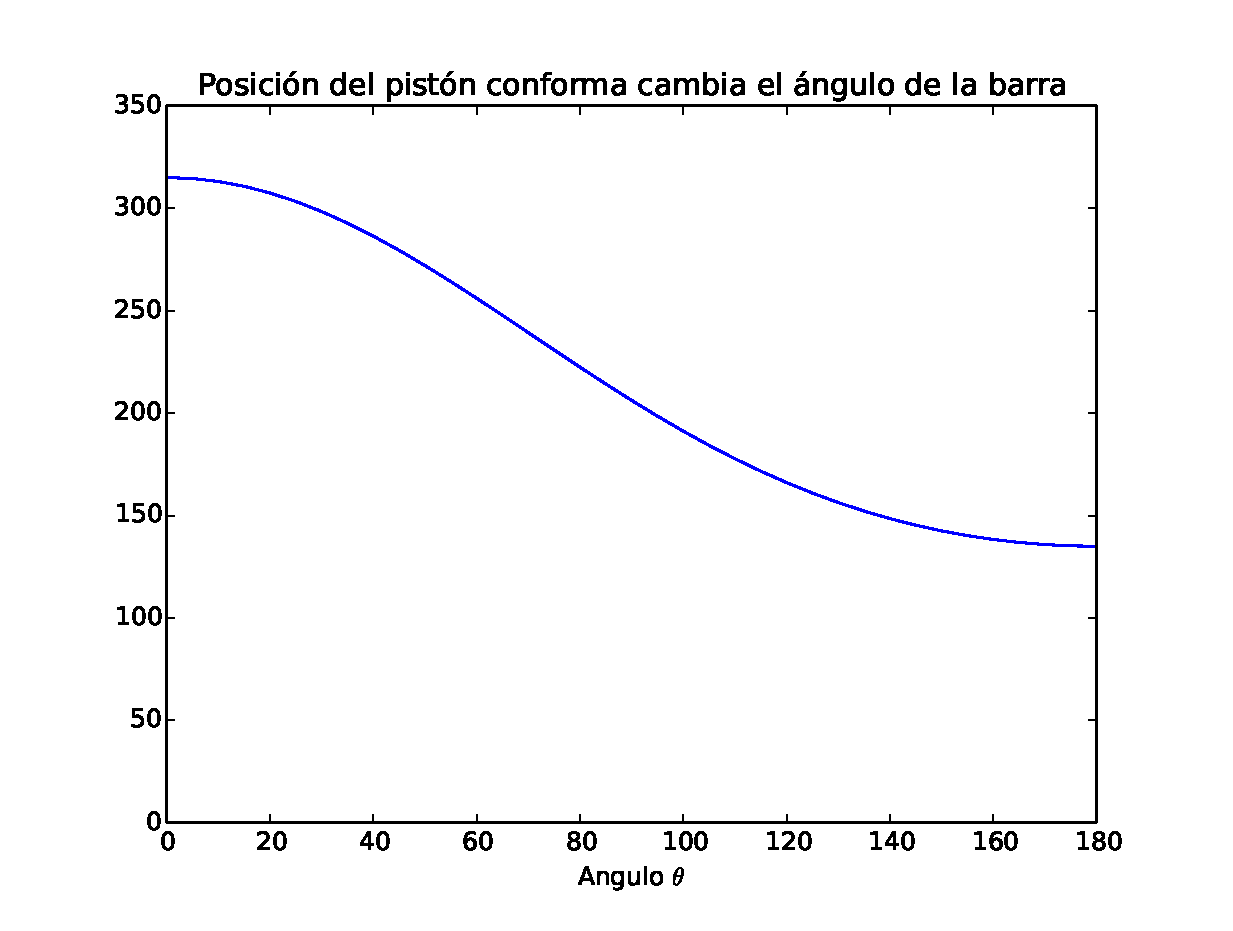
\includegraphics[scale=0.5]{Imagenes/Examen_2015_2_p3_01.eps}<1> 
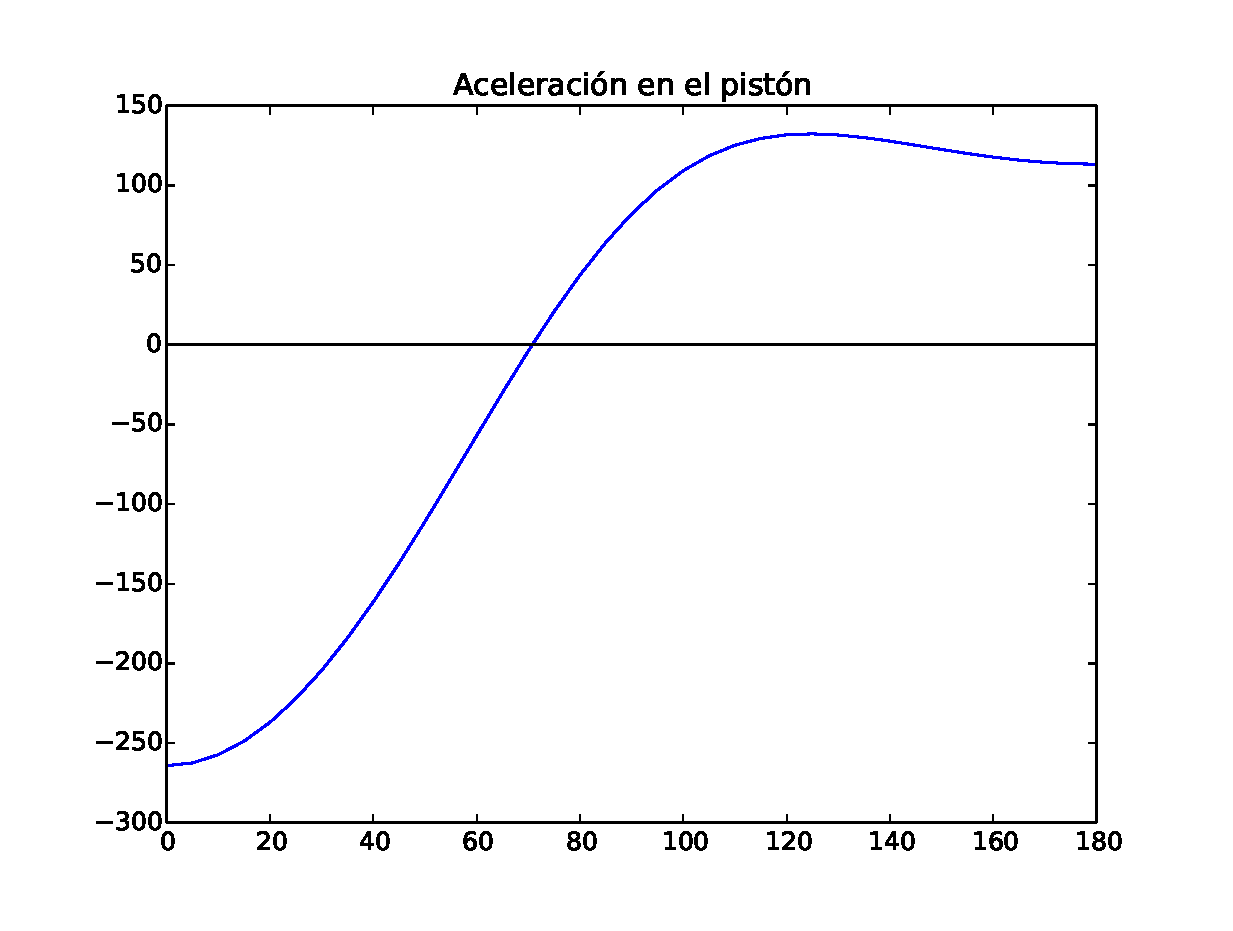
\includegraphics[scale=0.5]{Imagenes/Examen_2015_2_p3_02.eps}<2>
\end{figure}
\end{frame}
\begin{frame}
\frametitle{Problema 4}
Las estaciones de radar \textit{A} y \textit{B} están separadas por una distancia $a=500$ m; rastrean el avión \textit{C} registrando los ángulos $\alpha$ y $\beta$ en intervalos de un segundo. 
\begin{figure}[H]
	\centering
	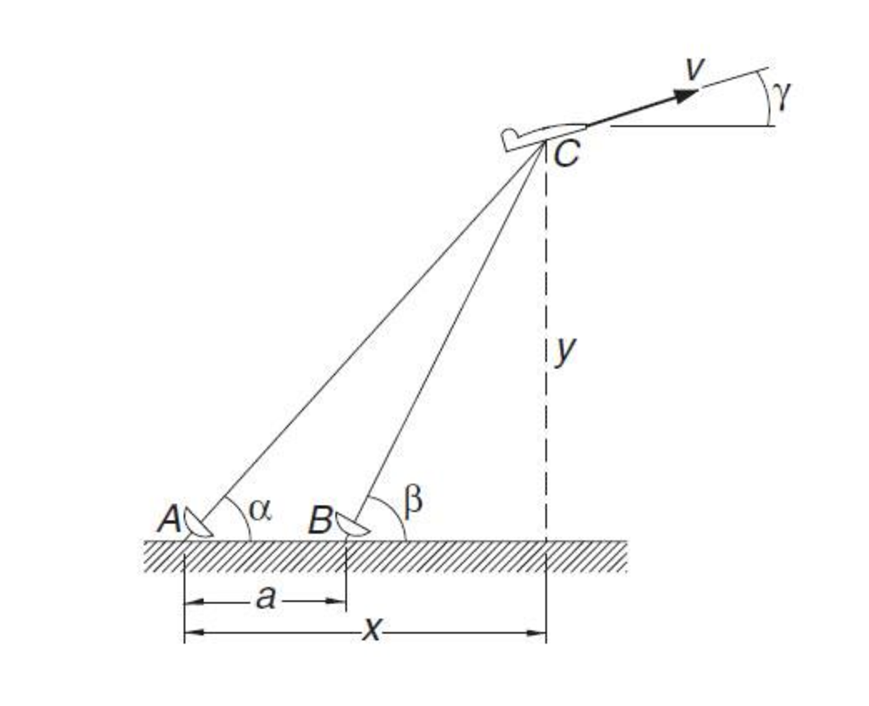
\includegraphics[scale=0.4]{Imagenes/ExamenFinal02_01.eps} 
	\caption{Estaciones de radar y el avión.}
\end{figure}
\end{frame}
\begin{frame}
Si hay tres lecturas sucesivas
\begin{center}
\begin{tabular}{c l l l }
t(s) & 9 & 10 & 11 \\ \hline
$\alpha$ & $54.80^{\circ}$ & $54.06^{\circ}$ & $53.34^{\circ}$ \\ \hline
$\beta$ & $65.59^{\circ}$ & $64.59^{\circ}$ & $63.62^{\circ}$
\end{tabular}
\end{center}
Calcula la velocidad $v$ del avión y el ángulo de subida $\gamma$ en $t=10$ segundos. Las coordenadas del avión las tomamos de
\[x = a \dfrac{\tan \beta}{tan \beta - tan \alpha} \hspace{1.5cm} y= a\dfrac{tan \alpha \tan \beta}{\tan \beta - \tan \alpha}\]
\end{frame}
\begin{frame}
Lo que podemos hacer es calcular $v_{x}$y $v_{y}$ en $t=10$ segundos, para luego obtener la velocidad
\[ v = \sqrt{v_{x}^{2} + v_{y}^{2}}\]
el ángulo de subida $\gamma$ resulta de
\[ \arctan \left( \dfrac{v_{y}}{v_{y}} \right)\]
así pues, tenemos que
\begin{eqnarray*}
v &=& 50.099 \mbox{ m/s} \\
\gamma &=& 15.14^{\circ}
\end{eqnarray*}
\end{frame}
\begin{frame}
\frametitle{Problema 5}
Obtén la aproximación por diferencias centrales de $f''(x)$ de orden $O(h^{4})$ aplicando la extrapolación de Richardson a la aproximación por diferencias centrales de orden $O(h^{2})$
\end{frame}
\begin{frame}
Conocemos $f''(x)$ por medio de la aproximación por diferencias centrales de orden $O(h^{2})$
\[ f''(x) = \dfrac{f(x+h)-2f(x)+f(x-h)}{h^{2}} + O(h^{2})\]
De la extrapolación de Richardson con $h_{2} = h_{1}/2$ tenemos el resultado
\[ G = \dfrac{2^{p} g\left( \frac{h_{1}}{2} \right) - g(h_{1})}{2^{p}-1} \]
\end{frame}
\begin{frame}
Haciendo $p=2$ y con el desarrollo de $G$, tenemos que la aproximación por diferencias centrales de $f''(x)$ de orden $O(h^{4}$ con la extrapolación de Richardson, resulta ser
\[ \begin{split}
 G &= \dfrac{1}{3h} \left[ 16 f \left( x + \dfrac{h_{1}}{2} \right) - f(x+h_{1}) - 30 f(x) + \right. \\
 &- \left. f(x-h_{1}) + 16 f \left( x - \dfrac{h_{1}}{2} \right) \right]
\end{split} \]
\end{frame}
\begin{frame}
\frametitle{Problema 6}
Obtén la primera aproximación por diferencias centrales para $f^{4}(x)$ a partir de la serie de Taylor.
\end{frame}
\begin{frame}
A partir del desarrollo en series de Taylor, tenemos que
\fontsize{10}{10}\selectfont
\begin{eqnarray*}
f(x+h) &=& f(x) + hf'(x) + \dfrac{h^{2}}{2!}f''(x) + \dfrac{h^{3}}{3!}f'''(x) + \dfrac{h^{4}}{4!}f^{4}(x) + \ldots \\
f(x-h) &=& f(x) - hf'(x) + \dfrac{h^{2}}{2!}f''(x) - \dfrac{h^{3}}{3!}f'''(x) + \dfrac{h^{4}}{4!}f^{4}(x) - \ldots \\
f(x+2h) &=& f(x) + 2hf'(x) + \dfrac{(2h)^{2}}{2!}f''(x) + \dfrac{(2h)^{3}}{3!}f'''(x) + \dfrac{(2h)^{4}}{4!}f^{4}(x) + \ldots \\
f(x-2h) &=& f(x) - 2hf'(x) + \dfrac{(2h)^{2}}{2!}f''(x) - \dfrac{(2h)^{3}}{3!}f'''(x) + \dfrac{(2h)^{4}}{4!}f^{4}(x) - \ldots
\end{eqnarray*}
\fontsize{14}{14}\selectfont
Haciendo el álgebra correspondiente, tenemos que
\end{frame}
\begin{frame}
La expresión para la primera aproximación por diferencias centrales para $f^{4}(x)$ es
\[ \begin{split}
 f^{4}(x) &=  \dfrac{1}{h^{4}} \left[ f(2x+2h) - 4f(x+h)+6f(x) + \right. \\
 &- \left. 4f(x-h)+f(x-2h) \right] \end{split} \]
\end{frame}
\section{Integración}
\begin{frame}
\frametitle{Problema 7}
Usa la regla del trapecio recursiva para evaluar
\[ \int_{0}^{\frac{\pi}{4}} ln(1 + \tan(x)) dx\]
Explica tus resultados.
\end{frame}
\begin{frame}
\frametitle{Resultados}
Usando diferentes valores para $k$
\begin{center}
\begin{tabular}{r | c | c}
k &  Integral & error \\ \hline
$1$ & $0.272198261$ & $0.00000$ \\ \hline
$5$ & $0.272198261$ & $0.00000$ \\ \hline
$10$ & $0.272198261$ & $0.00000$ \\ \hline
$15$ & $0.272198261$ & $0.00000$ \\ \hline
$20$ & $0.272198261$ & $0.00000$
\end{tabular}
\end{center}
\end{frame}
\begin{frame}
\frametitle{Problema 8}
La siguiente tabla indica la potencia $P$ propocionada por las ruedas de un carro como función de la velocidad $v$. Si la masa del carro es $m=2000$ kg, calcula el tiempo $\Delta t$ necesario para que el carro acelere de $1$ m/s a $6$ m/s. Usa la regla del trapecio para integrar.
\end{frame}
\begin{frame}
Tip:
\[ \Delta t = m \int_{1s}^{6s} \left( \dfrac{v}{P} \right) dv\]
que se puede obtener de la ley de Newton $F= m/(dv/dt)$ y por la definición de potencia, $P=Fv$.
\begin{center}
\begin{tabular}{c | c | c | c | c | c | c | c | c}
$v$ (m/s) & $0$ & $1.0$ & $1.8$ & $2.4$ & $3.5$ & $4.4$ & $5.1$ & $6.0$ \\ \hline
$P$ (kW)  & $0$ & $4.7$ & $12.2$ & $19.0$ & $31.8$ & $40.1$ & $43.8$ & $43.2$ 
\end{tabular}
\end{center}
\pause
El tiempo necesario para aumentar la velocidad es de: \textcolor{red}{1.6658 segundos}
\end{frame}
\begin{frame}
\frametitle{Problema 9}
La siguiente tabla proporciona el empuje $F$ del arco como función del desplazamiento $x$. Si la cuerda tiene un desplazamiento de $0.5$ m, calcula la velocidad de una flecha de $0.075$ kg, cuando sale del arco. Tip: la energía cinética de la flecha es igual al trabajo hecho al estirar la cuerda, que es:
\[ m \dfrac{v^{2}}{2} = \int_{0}^{0.5m} F dx\]
\end{frame}
\begin{frame}[fragile]
\frametitle{Tabla de datos}
\begin{center}
\begin{tabular}{c | c | c | c | c | c | c |}
$x$ (m) & 0.00 & 0.05 & 0.10 & 0.15 & 0.20 & 0.25  \\ \hline
$F$ (N)  & 0 & 37 & 71 & 104 & 134 & 161
\end{tabular}
\end{center}
\begin{center}
\begin{tabular}{c | c | c | c | c | c | }
$x$ (m) & 0.30 & 0.35 & 0.40 & 0.45 & 0.50 \\ \hline
$F$ (N)  & 185 & 207 & 225 & 239 & 250 
\end{tabular}
\end{center}
\begin{figure}
\centering
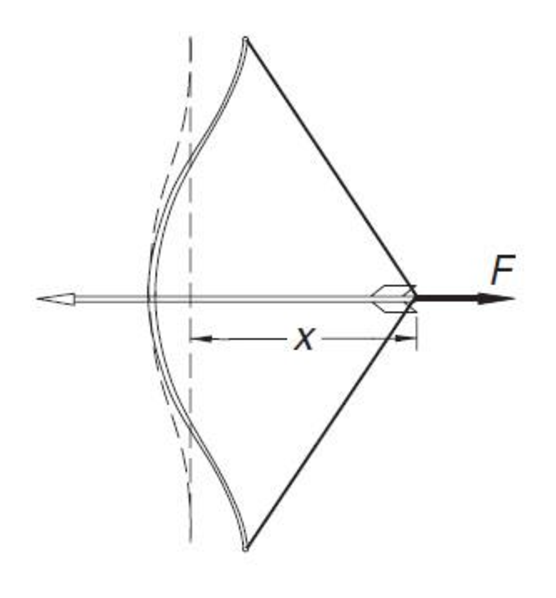
\includegraphics[scale=0.4]{Imagenes/Integral_01_Arco.eps} 
\end{figure}
\end{frame}
\begin{frame}[fragile]
Usando la regla extendida del trapecio y ajustando el valor del peso de la flecha, resulta que la velocidad de la flecha es: \textcolor{red}{$44.54$ m/s}
\end{frame}
\begin{frame}
El período de un péndulo de longitud $L$ es $\tau = 4 \sqrt{\frac{L}{g}} h(\theta_{0})$, donde $g$ es la aceleración debida a la gravedad, $\theta_{0}$, representa la amplitud angular y 
\[ h(\theta_{0}) =  \int_{0}^{\frac{\pi}{2}} \dfrac{d\theta}{\sqrt{1 - \sin^{2} \left( \frac{\theta_{0}}{2}\right) \sin^{2} \theta}} \]
Calcular $h(15^{\circ})$, $h(30^{\circ})$ y $h(45^{\circ})$; compara esos valores con $h(0^{\circ}) = \frac{\pi}{2}$ (la aproximación usada para pequeñas amplitudes)
\end{frame}
\begin{frame}
\frametitle{Resultados}
\begin{center}
\begin{tabular}{c | c | c}
$\theta$ & $h(\theta)$  & error \\ \hline
$15^{\circ}$ & $1.57755$ & $4.30058e-03$ \\ \hline
$30^{\circ}$ & $1.59814$ & $1.74088e-02$ \\ \hline
$45^{\circ}$ & $1.63359$ & $3.99733e-02$ 
\end{tabular}
\end{center}
\end{frame}
\end{document}